% -----------------------------------------------
% Template for ISMIR Papers
% 2015 version, based on previous ISMIR templates
% -----------------------------------------------

\documentclass{article}
\usepackage{ismir,amsmath,cite}
\usepackage{url}
\usepackage{graphicx}
\usepackage{color}
%\usepackage{hyperref}

\graphicspath{{figs/}}

% Title.
% ------
\title{Four Difficult Lessons on Automatic Chord Estimation}

% Two addresses
% --------------
%\twoauthors
%  {First author} {School \\ Department}
%  {Second author} {Company \\ Address}

% Three addresses
% --------------
\threeauthors
  {First author} {Affiliation1 \\ {\tt author1@ismir.net}}
  {Second author} {\bf Retain these fake authors in\\\bf submission to preserve the formatting}
  {Third author} {Affiliation3 \\ {\tt author3@ismir.net}}


\begin{document}
%
\maketitle
%
\begin{abstract}

Automatic chord estimation (ACE) is now a hallmark research topic in content-based music informatics, but like many other tasks, system performance appears to be converging to yet another glass ceiling.
Recently, two different large-vocabulary ACE systems were developed in the hopes that complex, data-driven models might significantly advance the state of the art.
While arguably achieving some of the highest results to date, both approaches plateau at the same level, well short of having solved the problem.
Therefore, this work explores the behavior of these two systems as a means of understanding obstacles and limitations in chord estimation, arriving at four difficult lessons:
one, music recordings that invalidate tacit assumptions about harmony and tonality result in erroneous and even misleading performance;
two, standard lexicons and comparison methods struggle to reflect the natural relationships between chords;
three, conventional approaches conflate the competing goals of recognition and transcription to some undefined degree;
and four, the perception of chords in real music can be highly subjective, making the very notion of ``ground truth'' annotations tenuous.
Synthesizing these observations, this paper offers possible remedies going forward, and concludes with some perspectives on the future of ACE research.

\end{abstract}


\section{Introduction}
\label{sec:introduction}

% Chord rec is standard in the community
Among the various subtopics in content-based music informatics, automatic chord estimation (ACE) has matured into a classic MIR challenge, receiving healthy attention from the research community for the better part of two decades.
%, people want / need
Complementing our natural sense of academic intrigue, the broader music learning public places a high demand on chord-based representations of popular music, as evidenced by large online communities surrounding websites like e-chords\footnote{\url{http://www.e-chords.com}} or Ultimate Guitar\footnote{\url{http://www.ultimate-guitar.com}}.
% ...but this is difficult
Given the prerequisite skill necessary to manually identify chords from recorded audio, there is considerable motivation to develop automated systems capable of reliably performing this task.


Following these motivations, the goal of ACE research is ---or, at least, has been--- to develop systems that produce ``good'' time-aligned sequence of chords from a given music signal.
Supplemented by efforts in data curation \cite{Burgoyne2011Billboard}, syntax standardization \cite{Harte2005XXX}, and evaluation \cite{Pauwels2013Evaluating}, the bulk of chord estimation research has concentrated on building better systems, mostly converging to a common architecture \cite{Cho2014Improved}:
%, diagrammed in Figure \ref{fig:basic_ace}
first, harmonic features, referred to as pitch class profiles (PCP) or \emph{chroma}, are extracted from short-time observations of the audio signal \cite{Fujishima1999Realtime};
these features may then be processed by any number of means, referred to in the literature as \emph{pre-filtering};
next, \emph{pattern matching} is performed independently over observations to measure the similarity between the signal and a set of pre-defined chord classes, yielding a time-varying posterior likelihood;
and finally, \emph{post-filtering} is applied to this chord class posterior, resulting in a sequence of chord labels over time.


Much time and energy has been invested in improving chroma features \cite{Mueller2010Towards}, while others have explored the use of multi-band chroma \cite{Mauch2010Simultaneous} or Tonnetz representations \cite{Lee2007Unified}.
% Some have tried feature learning
Acknowledging the challenges inherent to designing good features, Pachet et al pioneered work in automatic feature optimization \cite{Pachet2006Recognizing}, and more recently deep learning methods have been employed to learn robust Tonnetz features \cite{Humphrey2012Learning}.
Earlier methods focused on local smoothing, such as low-pass or median filtering as a form of pre-filtering \cite{Cho2010Exploring}, but more recently repetitive structure has been exploited for pre-filtering \cite{Cho2011Feature}.
Various classification strategies have been investigated such as binary templates \cite{Oudre2009Template}, Dirichlet distribution models \cite{Burgoyne2005Learning}, or Support Vector Machines (SVMs) \cite{Weller2009Structured}, but Gaussian Mixture Models (GMM) are by and large the most common feature modeling approach \cite{Cho2014Improved}.
Post-filtering methods, shown to significantly impact system performance \cite{Cho2010Exploring}, have become increasing more complex, ranging from Viterbi decoding \cite{Sheh2003Chord} to, more recently, Dynamic Bayesian Networks (DBNs) \cite{Mauch2010Approximate}, Conditional Random Fields \cite{Sumi2012Music}, or Recursive Neural Networks \cite{Boulanger2013Automatic}.


And yet, despite all this work, performance appears to be tapering off.
In addition to apparently beginning to over-fit the data used at MIREX, the application of larger datasets and chord vocabularies has further diminished state of the art performance.
Where do we go from here?
What are the limitations of this approach?
What can we learn from thorough error analysis?
This work proposes that it is worth pausing to consider that perhaps there is something else afoot.
% Not just about building a better mousetrap
This paper is organized as follows:
Section \ref{}
Section \ref{}


\section{ACE Research Methodology}

A generic research methodology for content-based music informatics looks something like the following:

\begin{enumerate}
\item Define the problem.
\item Collect data accordingly.
\item Build a solution.
\item Evaluate the model.
\item Iterate.
\end{enumerate}


\subsection{What is a ``chord''?}

% Attempts to define a chord
Despite their ubiquitous use in describing music, a practical definition of a chord is open to some interpretation.
For example, \cite{McVicar2013Machine} collects three possible definitions:

\begin{enumerate}
\item \emph{Everyone agrees that \emph{chord} is used for a group of musical tones.}
\item \emph{Two or more notes sounding simultaneously are known as a chord.}
\item \emph{Three or more pitches sounded simultaneously or functioning as if sounded simultaneously.}
\end{enumerate}

% Pitch and notes
\noindent Additionally, \cite{Harte2010Towards} expands the scope of (2) in order to describe \emph{all} tonal music, ``allow[ing] a chord to comprise zero or more notes.''
The various flavors of definitions begs an obvious question:
what makes the concept of a chord so hard to pin down?

% % Chord composition
% Much of this difficulty stems from the fact that the relative importance of the individual notes in a collection may change in different contexts.
% In practice, a chord is named based on three, potentially subjective, criteria:
% its root, its contributing intervals, and how these two relate to the perceived key.
% The one invariant property shared by all definitions named previously is the idea that a pitch collection may be understood as a single harmonic object.
% The time span over which this phenomena may unfold, however, is flexible.
%Therefore, as will be shown shortly, a chord may take a different name if any of these decisions are changed or re-weighted.

% Why is it so hard to define a chord? Let's look at some examples
\begin{figure}[t]
\centering
\includegraphics[width=0.8\columnwidth]{expanded_major}
\includegraphics[width=0.6\columnwidth]{nonchord_tones}
\caption{A stable F major chord played out over three time scales, as a true simultaneity, an arpeggiation, and four non-overlapping quarter notes; (bottom) a sustained C major chord is embellished by passing non-chord tones.}
\label{fig:harmonic_objects}
\end{figure}

% Expanded over time leads to the same chord
The inherent difficulty in defining a chord can be illustrated by two simple examples.
Consider the two short phrases notated in Figure \ref{fig:harmonic_objects}.
First, an \texttt{F:maj} chord is written as a true simultaneity, an arpeggiation, and as a series of non-overlapping quarter notes, respectively.
Here, the degree of overlap in time is expanded until it no longer exists, and yet the collection of notes will continue to function as a coherent harmonic object.
% True simultaneity doesn't always make a chord
On the other hand, the simultaneous sounding of different notes does not necessarily give rise to the perception of different chords, where a major triad is sustained under the first several degrees of its scale.
While three notes in the upper voice are contained in the \texttt{C:maj}, the others --the D, F, and A-- are referred to as ``nonchord'' tones.
These incompatible notes are explained away in the overall harmonic scene, as they fall on metrically weak beats, are comparatively short in duration, and quickly move to notes that \emph{are} in the chord.
%These embellishments do not contribute to the harmonic center of the phrase, and the bar can still be understood as a stable C major chord.


\subsection{Data Collections}\label{subsec:data}

% Actually, how you define a chord doesn't really matter; this is implicitly a function of the data you use.
In the absence of an explicit definition of a chord, one is adopted implicitly in the process of curating a set of chord annotations.
Definition of a chord and the chord annotations collected are indistinguishable.

\subsubsection{Ground Truth Datasets}

There are several chord annotation datasets available for research purposes.
The first major effort to curate reference chord annotations is referred to as the ``Isophonics'' dataset\footnote{\url{http://isophonics.net/content/reference-annotations}}.
Initially covering the entire 180-song discography of The Beatles, it has since expanded slightly;
of this additional content, 20 tracks by the band Queen are used here.
Two other large chord annotation datasets were publicly released in 2011, offering a more diverse musical palette.
The McGill \emph{Billboard} dataset consists of over 1000 annotations, of which more than 700 have been made public.
This project employed a rigorous sampling and annotation process, selecting songs from Billboard magazine's ``Hot 100'' charts spanning more than three decades.
The other, provided by the Music and Audio Research Lab (MARL) at NYU\footnote{\url{https://github.com/tmc323/Chord-Annotations}}, consists of 295 chord annotations performed by undergraduate music students;
195 tracks are drawn from the USPop dataset\footnote{\url{http://labrosa.ee.columbia.edu/projects/musicsim/uspop2002.html}}, and 100 from the RWC-Pop collection\footnote{\url{https://staff.aist.go.jp/m.goto/RWC-MDB/rwc-mdb-p.html}}, in the hopes that leveraging common MIR datasets might facilitate access within the community.
In all three cases, chord annotations are provided as ``ground truth,'' on the premise that the annotations represent the gold standard annotation.
%, and as such, employed a review process, where the transcriptions of one or more annotators were verified by different individuals.


\subsubsection{The Rock Corpus}

The majority of human-provided chord annotations are often singular, either being performed by one person or as the result of a review process to resolve disagreements.
Alternatively, the \emph{Rock Corpus} dataset, first introduced in \cite{deClercq2011Corpus}, is a set of 200 popular rock tracks with time-aligned chord and melody transcriptions performed by two expert musicians:
one, a pianist, and the other, a guitarist.
% This insight into musical expertise adds an interesting dimension to the inquiry when attempting to understand alternate interpretations by the annotators.
This collection of chord transcriptions has seen little use in the ACE literature, as its initial release lacked timing data for the transcriptions.
A subsequent release fixed this issue, however, in addition to doubling the size of the collection.
While previous efforts have sought to better understand the role of subjectivity in chord annotations \cite{Ni2013Understanding}, this dataset provides an opportunity to explore the behavior of ACE systems as a function of multiple reference transcriptions at a larger scale.


\subsection{Automatic Systems}
\label{subsec:systems}

There are a variety of chord algorithms out there.
We focus our investigation on two high-performing systems for which we are able to control for training and vocabulary.
These systems are reasonably different, and will hopefully provide different machine perspectives of the chord estimation problem.


\subsubsection{K-stream GMM-HMM with Multiband Chroma}

Following the lineage of automatic chord estimation systems, one system considered is that of \cite{Cho2014Improved}, referred to here as ``kHMM.''
A multiband chroma representation is computed from beat-synchronous audio analysis, producing four parallel chroma features.
Each is fit to a separate Gaussian Mixture Model (GMM) by rotating all chroma vectors and chord labels to C.
During inference, four separate observation likelihoods over all chord classes are obtained by circularly rotating the feature vector the GMM.
These four posteriors are then decoded jointly, using a k-stream HMM, resulting in a beat-aligned chord sequence.


\subsubsection{Deep Convolutional Neural Network}

Acknowledging both the limited representational power of GMMs and a similar trend that occurred in automatic speech recognition, a deep convolutional network is also considered \cite{Humphrey2015Fully}, referred to as ``DNN.''
Time-frequency patches of local contrast normalized constant-Q spectra, on the order of one second, are transformed by a fully-convolutional network.
Finding inspiration in the root-invariance strategy of GMM training, explicit weight-tying is achieved across roots such that all qualities develop the same internal representations, allowing the model to generalize to chords unseen during.
Taking inspiration from work in automatic speech recognition with deep networks, likelihood scaling is performed after training to control class bias resulting from the severe imbalance in the distribution of chords.
Finally, chord posteriors are decoded via the classic Viterbi algorithm, common among ACE research.


\subsection{Evaluation}

Expressed formally, the conventional approach to scoring an ACE system is a weighted measure of chord-symbol recall, $R_{W}$, between a reference, $\mathcal{R}$, and estimation, $\mathcal{E}$, chord sequence as a \emph{continuous} integral over time, summed over a collection of $N$ pairs:

\begin{equation}
\label{eq:recall_micro}
R_{W} = \frac{1}{S}\sum_{n=0}^{N-1}\int_{t=0}^{T_n}C(\mathcal{R}_n(t), \mathcal{E}_n(t))~dt
\end{equation}

\noindent Here, $C$ is a chord \emph{comparison} function, bounded on $[0, 1]$, $t$ is time, $n$ the index of the track in a collection, $T_n$ the duration of the $n^{th}$ track. $S$ corresponds to the cumulative amount of time, or \emph{support}, on which $C$ is defined, computed by a similar integral:

\begin{equation}
S = \sum_{n=0}^{N-1}\int_{t=0}^{T_n}(\mathcal{R}_n(t), \mathcal{E}_n(t) \in \Re)~dt
\end{equation}

Defining the normalization term $S$ separately is useful when comparing chord names, as it relaxes the assumption that the comparison function is defined everywhere.
Furthermore, setting the comparison function as a free variable allows for flexible evaluation of a system's outputs, and thus the focus on vocabulary can largely focus on the choice of comparison function, $C$.
The work presented here leverages \texttt{mir\_eval}, an open source evaluation toolbox providing a suite of chord comparison functions;
for more detail, we refer the curious reader to \cite{Raffel2014Eval}.


\section{Experimental Setup}
\label{sec:exp_setup}

The ground truth collections are merged for training and evaluation, totaling 1235 tracks.
Duplicates are then identified and removed to avoid potential data contamination during cross validation.
Each recording is checked against the EchoNest Analyze API\footnote{\url{http://developer.echonest.com/docs/v4}} and associated with its track and song identifiers, corresponding to the recording and work, respectively.
Uniqueness is defined at the level of a song ID to catch all possible conflicts, identifying 18 redundant tracks.
All but one is dropped for each collision, preferred in the order of ``Isophonics'', ``Billboard'', and ``MARL'', resulting in a final count of 1217 unique tracks.

For algorithmic parity, the two automatic systems addressed in Subsection \ref{subsec:systems} are trained with the same data partitions for 5-fold cross validation.
Both adopt the same common chord vocabulary, comprised of the thirteen most frequent chord qualities in all twelve pitch classes, in addition to the no-chord class, as in \cite{Cho2014Improved}.
Chords outside this strict vocabulary are ignored during training, rather than mapped to their nearest class approximation, as a means of exploring how the models generalize to such atypical instances.
Performance across the seven comparison rules are averaged over the five test splits for \emph{all} reference chord labels, given in Table \ref{tab:test_performance}.

\begin{table}[!t]
\scriptsize
\centering
\begin{tabular}{l||cc|c}
Rule      & $R_W$(Ref, DNN) & $R_W$(Ref, kHMM) & $R_W$(kHMM, DNN) \\
\hline
root      & 0.7894      & 0.8075       & 0.8398       \\
thirds    & 0.7570      & 0.7747       & 0.8148       \\
majmin    & 0.7589      & 0.7761       & 0.7980       \\
mirex     & 0.7691      & 0.7832       & 0.8060       \\
triads    & 0.7048      & 0.7205       & 0.7827       \\
sevenths  & 0.6197      & 0.6448       & 0.6913       \\
tetrads   & 0.5672      & 0.5880       & 0.6779       \\
v157      & 0.6493      & 0.6593       & 0.6779       \\
\hline
\end{tabular}
\caption{Weighted recall across comparison rules between the ground truth references and both models, respectively, as well as against each other.}
\label{tab:test_performance}
\end{table}

\begin{table}[!t]
\scriptsize
\centering
\begin{tabular}{l||c|cc}
Rule       & $R_W$(DT $|$ TdC) & $R_W$($\ast$, DNN) & $R_W$($\ast$, kHMM) \\
\hline
root        & 0.9318 & 0.7923 & 0.8353 \\
thirds      & 0.9031 & 0.7500 & 0.7845 \\
majmin      & 0.9054 & 0.7227 & 0.7657 \\
mirex       & 0.9024 & 0.7373 & 0.7757 \\
triads      & 0.8975 & 0.7186 & 0.7602 \\
sevenths    & 0.8424 & 0.5424 & 0.5950 \\
tetrads     & 0.8345 & 0.5395 & 0.5900 \\
v157        & 0.8381 & 0.5393 & 0.5903 \\
\hline
\end{tabular}
\caption{Weighted recall across comparison rules for the two human annotators, and the better match of each against the two automatic systems.}
\label{tab:rc_performance}
\end{table}

At first glance, the averaged statistics for each model against the reference annotations would seem to indicate that the two systems are roughly equivalent, with the kHMM system outperforming the DNN by a small margin.
Unsurprisingly, the machine estimations perform best at the root recall, and drop as the comparison rules include greater specificity.
However, as shown by the comparing the estimations in the third column, these two systems arrive at similar overall performance despite behaving quite differently.
In fact, the two automatic systems agree with each other only slightly more than either does with the ground truth.
Therefore, it will be valuable to not only investigate where the estimated chord sequences differ from the reference independently, but also how these estimated sequences differ from each other.


Similarly, quantitative results are given for both systems over the Rock Corpus data in Table \ref{tab:rc_performance}, with two notable caveats.
First, it is not immediately clear how to best use multiple perspectives when evaluating the machine estimations.
As this work is more concerned with general trends than establishing state of the art benchmarks, the best matching reference-estimation pair is chosen at the track level and used in the weighted average.
Additionally, it should be noted that the vocabulary of chords used in the Rock Corpus reference annotations is a smaller subset than that produced by the models.
This is likely reflected in the overall performance, where both systems achieve similar performance to the ground truth data at roots and thirds, but seem to fare far worse on the larger vocabulary metrics as result of over-estimating chords that could never be strictly right.
These considerations aside, it is curious to observe a non-negligible degree of disagreement between the two human perspectives.
Though hardly definitive, this helps establish a sense of what a natural performance ceiling might look like in ACE evaluation, with more than a $15\%$discrepancy in the tetrads condition.
That said, these results also seem to indicate that there is certainly room for improvement in these systems.

% Want to shine light on what these errors might be, and how to possibly improve them.
While overall recall gives a good general measure of system performance, we are particularly interested in developing a more nuanced understanding of how these systems behave.
% but it is likely that they don't tell the whole story,
% Therefore, it is necessary explore performance at a more granular level to untangle what factors contribute to these numbers.
Track-wise analysis is informative in this instance, due to the strong relationship between chords and harmony internal to a song.
Errors and other kinds of noteworthy behavior should be well-localized within a track as a result, making it easier to draw broader conclusions from the data.

\begin{figure}[!t]
\centering
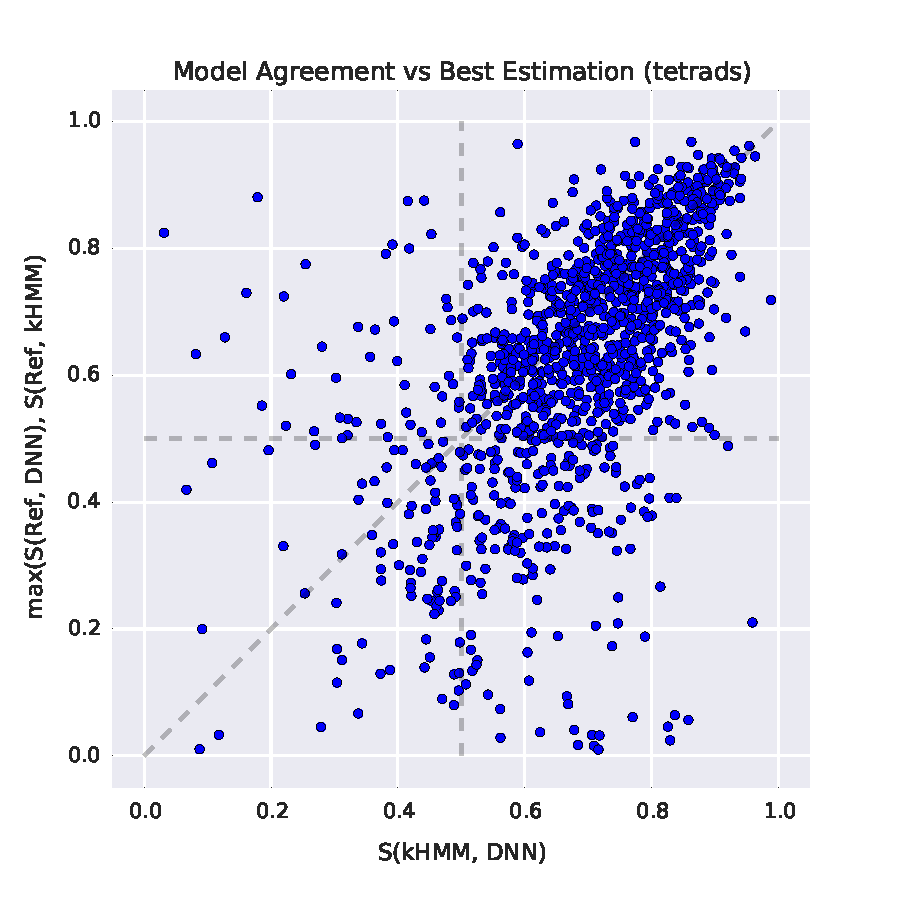
\includegraphics[width=\columnwidth]{model_agreement-vs-best_est}
\caption{Trackwise recall for the ``tetrads'' rule over the ground truth data, illustrating \emph{model} agreement versus the better match between the reference and estimated annotations.}
\label{fig:model_agreement}
\end{figure}

\begin{figure}[!t]
\centering
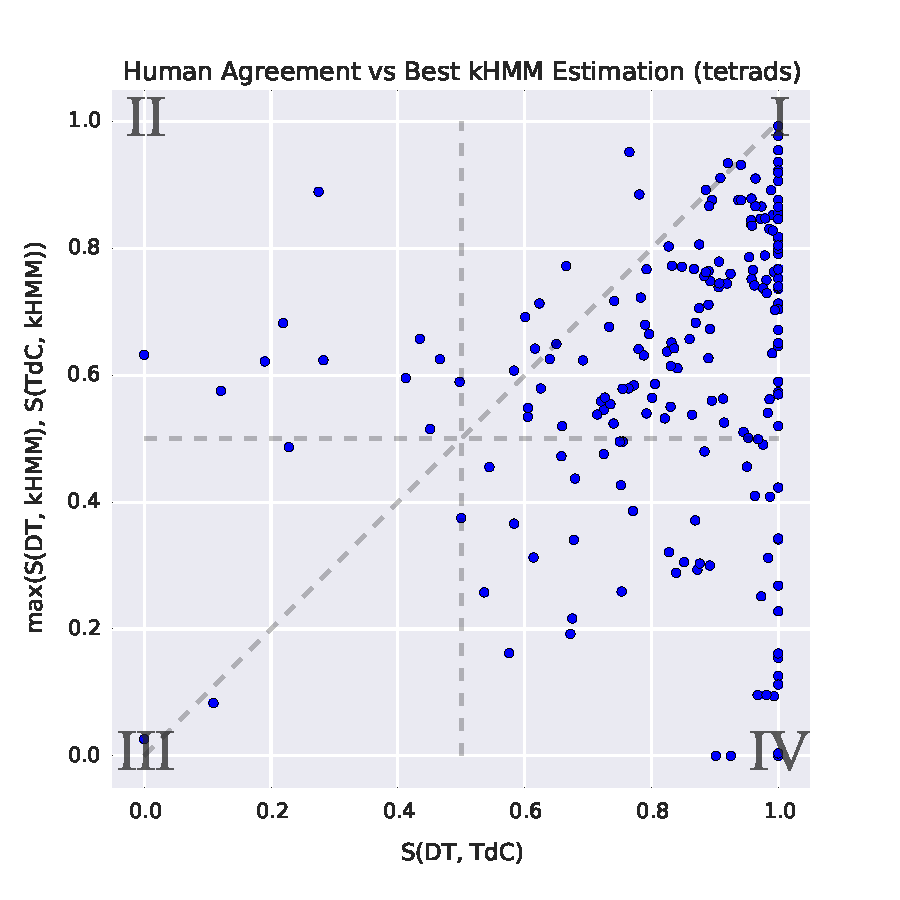
\includegraphics[width=\columnwidth]{human_agreement-vs-best_kHMM_est}
\caption{Trackwise recall for the ``tetrads'' rule over the Rock Corpus data, illustrating annotator agreement versus the better match between the two reference and kHMM annotations.}
\label{fig:annotator_agreement}
\end{figure}

\begin{figure*}[t!]
\centering
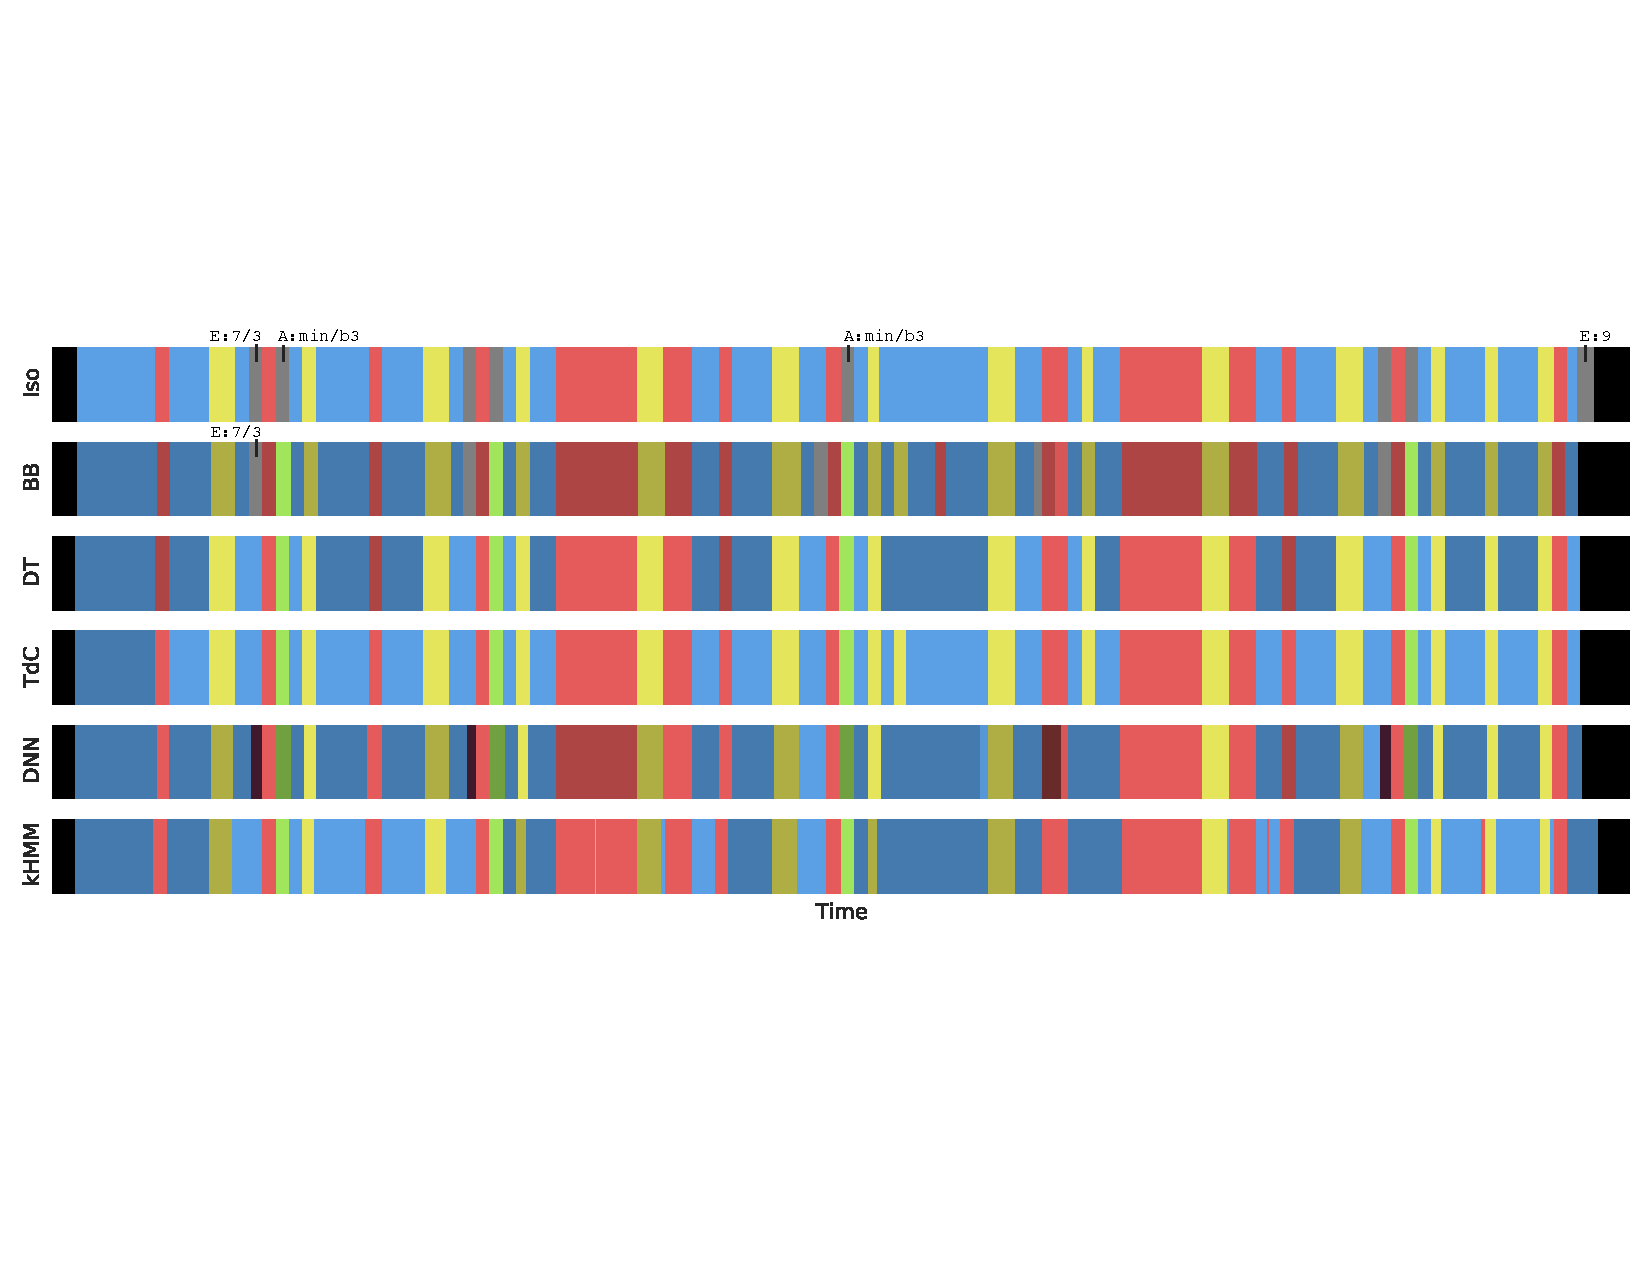
\includegraphics[width=\textwidth]{TROSSUK149E3AE03BD_annotations_mkup2}
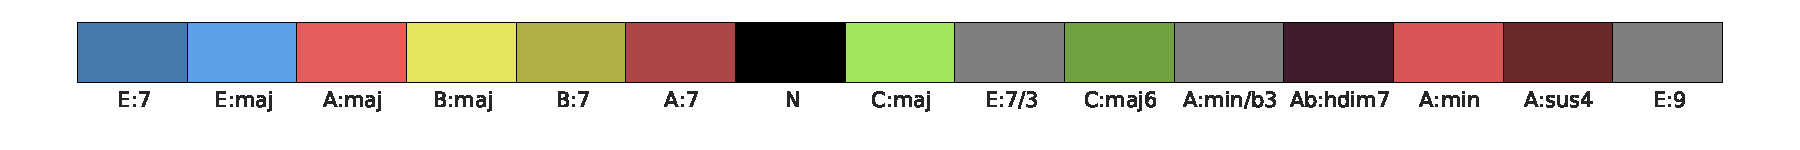
\includegraphics[width=\textwidth]{TROSSUK149E3AE03BD_legend}
\caption{Six perspectives on ``I Saw Her Standing There'', by \emph{The Beatles}, according to Isophonics (Iso), Billboard (BB), David Temperley (DT), Trevor deClercq (TdC), the Deep Neural Network (DNN), and the k-stream HMM (kHMM).}
\label{fig:beatles}
\end{figure*}


% Ground truth trackwise
First, leveraging the ground truth data, Figure \ref{fig:model_agreement} compares the agreement between machine estimations, along $x$, with the better estimated annotation for the given reference, along $y$.
This comparison is motivated by a three-fold hypothesis:
one, tracks that result in similar incorrect estimations present some kind of greater challenge, and it would be beneficial to know that might be;
two, tracks that only one algorithm can get ``right'' contain understandable confusions;
and three, tracks where both algorithms produce poor estimations, and yet \emph{neither} agree, are particularly curious and warrant further inspection.
Partitioning the plot at its midpoints yields four quadrants, enumerated I-IV in a counterclockwise manner from the upper right, each corresponding to a different kind of behavior:
Quadrant I, $(x > 0.5, y > 0.5)$, in which all annotations agree;
Quadrant II, $(x < 0.5, y > 0.5)$, in which one estimation matches the reference better than the other;
Quadrant III, $(x < 0.5, y < 0.5)$, in which all annotations disagree;
and finally, Quadrant IV, $(x > 0.5, y < 0.5)$, in which the estimations agree more with each other than the reference.


% Rock corpus
A similar comparison is made over the Rock Corpus dataset, given in Figure \ref{fig:annotator_agreement}, where \emph{annotator} agreement, along $x$, is shown against the agreement of the best matching reference for a given estimation, along $y$.
As an analog to the previous plot, only a single estimation (kHMM) is considered, offering a comparable three-part hypothesis:
one, tracks with an estimated annotation that fails to match either human perspective likely identify room for improvement;
two, annotator disagreement in the presence of a matching estimation highlights a subjective annotation;
and three, disagreement between all annotations is suspicious and should be explored.
A quadrant partition consistent with the previous plot yields a similar interpretation, exchanging dual estimations for dual references.


\section{Understanding Performance, in Four Parts}
\label{sec:data_analysis}

Having built these two trackwise representations to help organize over 1400 tracks, we can now poke around and identify things.
Using the trackwise plots to identify interesting datapoints worthy of qualitative inspection.
Dig through the estimations, look at errors.
Arrive at a variety of observations that are outlined here.

A particularly dense example is given in Figure \ref{fig:beatles}, which happens to intersect the Isophonics, Billboard, and Rock Corpus datasets, resulting in four human and two machine estimations.



% Content Validity
\subsection{Harmonic Validity}
\label{subsec:validity}

For both Figures \ref{fig:model_agreement} and \ref{fig:model_agreement}, Quadrant III ---the condition where all annotations disagree--- serves to identify tracks that contribute a large source of error to overall performance, but on which no one can agree.
Investigating these tracks further results in two general discoveries, both related to the notion of harmonic validity.

% Alternatively, systems are sensitive to tuning.
% This is another easy way to pick up goose eggs during evaluation.
% While the outputs might be spot on and even useful to a human, sensitivity to absolute chord spelling fails to
% This motivates harmonic, Roman numeral analysis as a slightly different formulation of the task; decouple tuning from function.
% While not all chord datasets contain this information, Billboard and Isophonics do.

The first issue stems from issues of tuning and intonation.
A number of tracks are not tuned to A440, in some instances varying by more than a quarter-tone:
for example, ``Stand By Me'' by Jimmy Ruffin, ``I'll Tumble 4 Ya'' by \emph{The Culture Club}, ``Every Breath You Take'' by \emph{The Police}, or ``Nowhere to Run'' by Martha Reeves and the Vandellas.
As a result, the estimated annotations differ from the reference by a half-step, and yet yield recall scores near zero, often only getting the ``no-chords'' in the track correct.
While the importance of tuning has been discussed previously in ACE research, this raises two interesting questions.
Is it a meaningful obstacle to force automatic systems to compensate for imprecise tuning, or a necessary assumption given the task of estimating absolute chord names?
And furthermore, should evaluation measures be able to characterize ``good'' annotations that happen to be agnostic to key?

% Not all music is well described by chords.
The second, and far more interesting, observation, has to do with the fact that some tracks considered arguably do not have valid chord transcriptions.
While a few songs by \emph{The Beatles} have been known by those in the ACE community to be of questionable relevance, such as ``Revolution 9,'' ``Love You To,'' or ``Within You, Without You'', error analysis here reveals a greater number of tracks across a variety of genres:
for example, ``Brass Monkey'' by \emph{The Beastie Boys}, ``I, Me, \& Myself'' by \emph{de la Soul}, ``Don't Push'' by \emph{Sublime}, ``Get Up (I Feel Like Being a Sex Machine'' by James Brown, or ``I Wanna Take You Higher'' by Tina and Ike Turner.
This realization motivates the notion that the harmonic language of chords may not be applicable for all kinds of music, and that using such songs for evaluation may lead to erroneous or misleading results.


\subsection{Labels, Lexicons, \& the Limits of Flat Classification}

% Syntax yo
As discussed in \ref{sec:chord_syntax}, it is a particular nuance of chord notation that the space of valid spellings is effectively infinite.
To constrain the complexity of the task at hand, ACE systems are traditionally designed to estimate chords from a finite \emph{vocabulary}, defined \emph{a priori}.
This simplification reduces the chord estimation to a classification problem, where all observations are assigned to one of $K$ chord \emph{classes}.

Comparing chords in label space is bonkers.
Mappings or resolutions effectively quantize chords to a one-hot encoding.
These can be thought of as mapping chords to bit vectors and then testing for equivalence.
This is the wrong representation.

One, chords are inherently hierarchical, and this approach to resolution discards these relationships.
Flat classification problems ---those in which different classes are conceptually independent--- are built on the assumption of mutually exclusive relationships.
In other words, assignment to one class precludes the valid assignment to any other classes considered.
For example, ``cat'' and ``dog'' are mutually exclusive classes of ``animal'', but ``cat'' and ``mammal'' are not.
Returning to chords, \texttt{C:dim7} and \texttt{C:maj} are clearly mutually exclusive classes, but it is difficult to say the same of \texttt{C:maj7} and \texttt{C:maj}, as the former \emph{contains} the latter.

Two, the flexibility of the standard Harte syntax can be abused for ambiguous chords, and it isn't clear what to do with these labels.

Occurrence of bizarre chord spellings in the data:
Should these even exist?



Chords with bass intervals other than the root should be discarded from chord mapping strategies.
Otherwise, this will only introduce noise.


\subsection{Conflicting Problem Definitions}

The former is literal, the latter is anything but.
In a recognition problem, silence is always no-chord, because nothing is playing.
Transcription, on the other hand, is attempting to assign labels to regions, and is closer to segmentation than classic approaches to chord estimation.
It is easy to find instances of both in the data.

Unfortunately, reference datasets contain annotations of both styles, and sometimes internally to the same annotation.
Over-specified chords are mostly indicative of a recognition problem, and finds an ambiguous middle ground between harmonic analysis and pitch recognition.
Alternatively, there are plenty of instances in which annotators make transcriptions decisions.
Nirvana -- all apologies.


\subsection{``There is No Spoon,'' or Subjectivity in Chord Annotation}

Known issue, Ni and company \cite{Ni2013Understanding}.
Not enough attention is being drawn to this observation.
How can we objectively quantify a subjective task?

\begin{table*}[!t]
% increase table row spacing, adjust to taste
% \renewcommand{\arraystretch}{1.4}
% if using array.sty, it might be a good idea to tweak the value of
% \extrarowheight as needed to properly center the text within the cells
\small
\centering
\begin{tabular}{ c || c c c c | c c c c |}
Ver. & \multicolumn{4}{c}{Chord Sequence} & Score & Ratings & Views \\
 \hline
 Billboard & \texttt{D:maj} & \texttt{A:sus4(b7)} & \texttt{B:min7} & \texttt{G:maj9} & --- & --- & --- \\
 MARL & \texttt{D:maj} & \texttt{D:maj/5} & \texttt{D:maj6/6} & \texttt{D:maj(4)/4} & --- & --- & --- \\
 DT & \texttt{D:maj} & \texttt{A:maj} & \texttt{B:min} & \texttt{G:maj} & --- & --- & --- \\
 TdC & \texttt{D:maj} & \texttt{A:maj} & \texttt{B:min} & \texttt{G:maj} & --- & --- & --- \\
\hline
DNN & \texttt{D:maj} & \texttt{A:sus4} & \texttt{B:min7} & \texttt{G:maj7} & --- & --- & --- \\
kHMM & \texttt{D:maj} & \texttt{A:sus4} & \texttt{B:min} & \texttt{G:maj} & --- & --- & --- \\
\hline
1 & \texttt{D:maj} & \texttt{A:maj} & \texttt{B:min} & \texttt{G:maj} & 4/5 & 193 & 1,985,878 \\
2 & \texttt{D:5} & \texttt{A:sus4} & \texttt{B:min7} & \texttt{G:maj} & 5/5 & 11 & 184,611 \\
$3^*$ & \texttt{D:maj} & \texttt{A:maj} & \texttt{B:min} & \texttt{G:maj} & 4/5 & 23 & 188,152 \\
$4^*$ & \texttt{D:maj} & \texttt{A:maj} & \texttt{B:min} & \texttt{G:maj7} & 4/5 & 14 & 84,825 \\
$5^*$ & \texttt{D:maj} & \texttt{A:maj} & \texttt{B:min} & \texttt{G:maj} & 5/5 & 248 & 338,222 \\
6 & \texttt{D:5} & \texttt{A:5} & \texttt{D:5/B} & \texttt{G:5} & 5/5 & 5 & 16,208 \\
\hline
\end{tabular}
\caption{Various interpretations of the verse from ``With or Without You'' by \emph{U2}, comparing the reference annotations and automatic estimations with six interpretations from a popular guitar tablature website; a raised asterisk indicates the transcription is given relative to a capo, and transposed to the actual key here.}
\label{tab:wowu_chords}
\end{table*}

With or Without You
stuff and things


% \begin{figure*}[t]
% \centering
% \includegraphics[width=0.9\textwidth]{rc_TRJAZCU14A0814BC9D_annotations}
% \includegraphics[width=0.9\textwidth]{rc_TRJAZCU14A0814BC9D_legend}
% \caption{``All Apologies'', by Nirvana -- An instance from the \emph{Rock Corpus}, illustrating the role subjectivity can play in annotation and evaluation.}
% \label{fig:apologies}
% \end{figure*}




\section{Conclusions}

In this work, the application of deep learning to large-vocabulary ACE is thoroughly explored, advancing the state of the art using standard evaluation methods.
Arguably of more importance, both the behavior of the resulting systems and the data used for development are explored in rigorous detail.
Our results show that the state of the art may have truly hit a glass ceiling, due to the conventional assumption that ``ground truth'' data can be obtained for what is, at times, an unavoidably subjective task.
This challenge is further compounded by approaches to prediction and evaluation, which attempt to perform flat classification of a hierarchically structured chord taxonomy.
Thus, while there certainly remains room for improvement, error analysis indicates that the vast majority of error in modern chord recognition systems is a result of invalid assumptions baked into the very question being asked.

Notably, four issues with current chord estimation methodology have been identified in this work.
One, it seems necessary that computational models, and especially those that estimate a large number of chord types, embrace structured outputs;
one-of-$K$ class encoding schemes introuduce unnecessary complexity between what are naturally hierarchical relationships.
Two, there is value in distinguish between the two tasks at hand, being chord recognition ---I am playing this \emph{exact} chord shape on guitar--- and chord transcription ---finding the best chord label to describe this harmonically homogenous region of music--- and how this intent is conveyed to the authors of reference annotations.
Three, as championed by \cite{Mauch}, chord transcription would certainly seem to benefit from explicit segmentation, rather than letting such boundaries between regions of harmonic stability result implicitly from post-filtering algorithms, i.e. Viterbi.
Lastly, the all-too-often subjective nature of chord labeling needs to be acknowledged in the process of curating reference data, and the human labeling task should average or combine multiple perspectives rather than attempt to yield canonical ``expert'' references.


% \section{Citations}

% All bibliographical references should be listed at the end,
% inside a section named ``REFERENCES,'' numbered and in alphabetical order.
% All references listed should be cited in the text.
% When referring to a document, type the number in square brackets
% \cite{Author:00}, or for a range \cite{Author:00,Someone:10,Someone:04}.

% For bibtex users:
\bibliography{ISMIR2015template}

% For non bibtex users:
%\begin{thebibliography}{citations}
%
%\bibitem {Author:00}
%E. Author.
%``The Title of the Conference Paper,''
%{\it Proceedings of the International Symposium
%on Music Information Retrieval}, pp.~000--111, 2000.
%
%\bibitem{Someone:10}
%A. Someone, B. Someone, and C. Someone.
%``The Title of the Journal Paper,''
%{\it Journal of New Music Research},
%Vol.~A, No.~B, pp.~111--222, 2010.
%
%\bibitem{Someone:04} X. Someone and Y. Someone. {\it Title of the Book},
%    Editorial Acme, Porto, 2012.
%
%\end{thebibliography}

\end{document}
